\chapter{Trabajo Previo}

Siguiendo las definiciones dadas por Kennicutt el at. \cite{Kennicutt}, el término \textbf{nube molecular} se refiere a una estructura en el medio interestelar (ISM \textit{interstellar medium}) separada de sus alrededores por el rápido cambio de alguna propiedad, tales como la presión, densidad o estados químicos.

Las nubes tienen una estructura compleja, pero los astrónomos teóricos identifican dos estructuras principales: \textbf{Clumps}, entendidos como zonas de alta emisión dentro de un \textit{cluster}; \textbf{Núcleos}, entendidos como zonas de alta emisión dentro de estrellas individuales o binarias. Tales nubes moleculares están básicamente compuestas de gas y polvo, siendo los gases más abundantes el hidrógeno molecular $H_2$, $CO$, $H_2O$ y otras moléculas más complejas.

El gas y polvo interior de tales nubes se distribuye en una componente difusa, al interior de la cual hay filamentos de gas más denso en diversas direcciones, con composición química y propiedades físicas definidas. Dentro de tales filamentos se pueden encontrar los \textit{Núcleos} que se caracterizan por ser poco masivos pero muy densos, y los \textit{Clumps} que se caracterizan por ser regiones de mayor densidad, y están acotados por alguna propiedad.

\begin{figure}[htpb!]
\centering
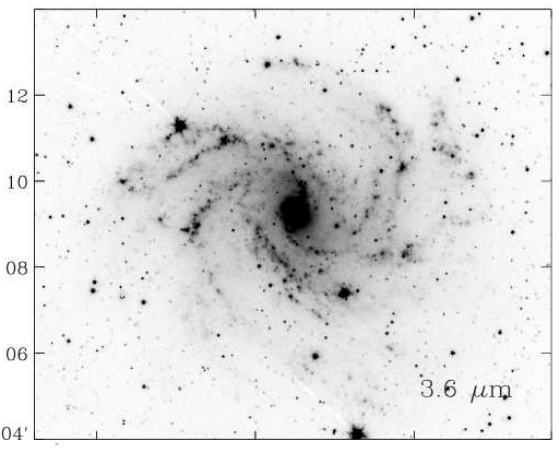
\includegraphics[width=9cm]{ngc}
\caption{Montaje de imágenes infrarrojas de NGC6946 desde \textit{Spitzer} y \textit{Herschel} (Fuente: \cite{Williams})}
\label{fig:cf}
\end{figure}

En las secciones siguientes se explican los principales algoritmos utilizados hoy en día, para la identificación de estructuras del tipo \textit{clump}.




\section{GaussClump}
Este método propuesto por Stutzki et al. \cite{Stutzki} y fue uno de los primeros en abordar de forma satisfactoria el problema de la identificación automática de clumps en cubos espectroscópicos. Como se explica y analiza también en Kramer et al. \cite{Kramer}, la idea principal de este método es ajustar perfiles Gaussianos que mejor ajusten cada uno de los peaks de emisión presentes en los datos. La razón de ocupar funciones Gaussianas sobre alguna otra opción, es debido a que observaciones de emisiones de algunas de las moléculas más frecuentes en nubes moleculares, han mostrado que su distribución de intensidad tiene forma de campana de Gauss.

El algoritmo iterativamente busca el máximo \textit{peak} de emisión actual, y determina la función gaussiana que mejor se ajusta a tal emisión y la región que lo rodea. Tal procedimiento consiste en determinar la intensidad del peak $a_0$, el centro $\mu=(\mu_x, \mu_y, \mu_z)$, los anchos por cada eje $(\sigma_x^2, \sigma_y^2, \sigma_z^2)$ y las orientaciones de cada eje $(\theta_x, \theta_y, \theta_z)$ de la Gaussiana, por medio de un proceso de minimización del error cuadrático. La función ajustada es agregada a un catálogo de salida y es restada del cubo de datos original, generando un cubo residual que será la entrada de la próxima iteración. Cómo resultado se obtienen un conjunto de Gaussianas con diferentes forma, posiciones, intensidades y orientaciones, que sumadas al ruido de fondo (residual final del proceso iterativo) permiten reconstruir (aproximadamente) el cubo espectroscópico original.


La función $\chi^2$ (notación utilizada en \cite{Stutzki}) a minimizar en cada iteración tiene varios componentes. En su forma más general puede ser escrita como:
\begin{align}
    \chi^2 = \sum \omega_i (Y_i - Y_i^{\text{fit}})^2 + s_0 \sum \omega_i \mathcal{F}(Y_i^{\text{fit}}- Y_i) + s_a (a_0 + b_0 - Y^{\text{max}})^2 + s_c ||\boldsymbol{\mu - \mu^{\text{max}}}||_2,
\end{align}
en donde cada uno de los términos tiene el siguiente significado (los parámetros $(s_0, s_a, s_c)$ permiten definir los pesos relativos de cada término dentro de $\chi^2$):
\begin{enumerate}
    \item $\displaystyle \sum \omega_i (Y_i - Y_i^{\text{fit}})^2$ es el término estándar de error cuadrático, donde $Y_i$ corresponden a las observaciones de intensidad, y $Y_i^{\text{fit}}$ a la función a ajustar, e $\omega_i$ son los pesos dados a cada observación.
    \item $\displaystyle \sum \omega_i \mathcal{F}(Y_i^{\text{fit}}-Y_i)$ penaliza los puntos en donde la función a ajustar sobrepasa a los valores observados, forzando de este modo a las Gaussianas a permanecer por debajo de los valores de la data. La función $\mathcal{F}$ es elegida como $\mathcal{F}(x)=\exp(x)$ en \cite{Stutzki}, mientras que en \cite{Kramer} se usa $\mathcal{F}(x) = (0 \text{ para } x\leq 0; \ x^2 \text{ para } x>0)$.
    \item En $(a_0 + b_0 - Y^{\text{max}})^2$, $a_0$ es el valor peak de la Gaussiana y $b_0$ es el nivel de base (definido como un múltiplo del RMS de la data). El objetivo de este es mantener el \textit{peak de amplitud} de la gaussiana ajustada cercano el peak observado $Y^{\text{max}}$.
    \item $||\boldsymbol{\mu - \mu^{\text{max}}}||_2$ es para forzar que el centro del clump observado y el centro la Gaussiana ajustada esten cercanos.
\end{enumerate}

En este algoritmo cada Gaussiana sustraída es considerada un clump de emisión individual, y debido a que entre las Gaussianas puede existir traslape, entonces es posible que un mismo píxel sea asignado a más de un clump. Esta característica distingue a este algoritmo de los otros métodos de identificación de clumps que siguen a continuación.



\section{ClumpFind}
Un enfoque totalmente distinto fue propuesto por Williams el al. \cite{Williams}. Este está inspirado en cómo los humanos detectan estructuras dentro de una imagen bidimensional; El ojo humano humano descompone mapas bidimensionales en estructuras isoladas determinando contornos de nivel, siguiendo de manera gradual desde los contornos de más alto nivel hacia lo más bajos, en donde se mezclan las distintas estructuras.

Del mismo modo \textit{ClumpFind} funciona contorneado la data en múltiplos del RMS del ruido de la observación, esto es, genera una serie de intervalos de intensidades (cada uno de ancho igual a un múltiplo del RMS anterior) en lo cuales se buscan estructuras isoladas (clumps). Este trabaja iterativamente iniciando en el nivel más alto (aquel que contiene al \text{peak}) y bajando de forma secuencial hacia los niveles más bajos, buscando en cada nivel las estructuras isoladas, es decir, los conjuntos de píxeles que no están conectados entre sí. Luego si la estructura/clump encontrado a un nivel dado, está conectado con un clump identificado en el nivel superior, entonces ambos corresponden a un mismo clump y se les asigna un mismo identificador. En caso contrario (el clump identificado en este nivel no está conectado con ninguno en el nivel superior) se define este como un nuevo clump encontrado.

Una situación especial se dá cuando un clump encontrado en un nivel está conectado con más de un clump en el nivel superior. Este es el caso de emisiones combinadas o conjuntas de dos clumps cercanos. En tales casos, tal estructura es separada asignando los píxeles que contiene, a cada uno de los clumps de los niveles superiores según un criterio, siendo el más común el conocido \textit{friends of friends}, que asigna un píxel según la cantidad de pixeles vecinos que pertenecen a cada clump (\textit{al con más amigos}).

\begin{figure}[htpb!]
\centering
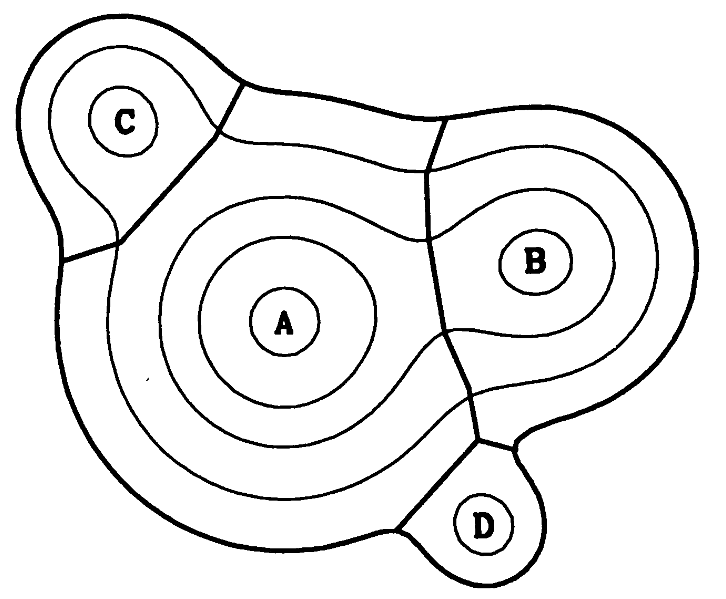
\includegraphics[width=6cm]{cf}
\caption{Resultados de ClumpFind en data 2D (Fuente: \cite{Williams})}
\label{fig:cf}
\end{figure}

Como resultado este algoritmo produce el \textit{Clump Assignment Array} o CAA, que es un arreglo de las mismas dimensiones de los datos de entrada, en el cual cada pixel tiene asignado el identificador del clump al que pertenece, como se muestra en la Figura \ref{fig:cf}. Una característica importante que distingue ClumpFind del resto de algoritmos, es que no realiza supuestos a priori acerca del perfil de los clumps, y por lo tanto los clumps encontrados pueden tener cualquier forma.



\section{FellWalker}
Un algoritmo más reciente corresponde al desarrollado por Berry et al. \cite{Berry}. Este está basado en el algoritmo de optimización \textit{Hill-Climbing}, aprovechando la propiedad de estancamiento en óptimos locales, para determinar los peaks de emisión locales y de este modo definir un nuevo clump. Al igual que ClumpFind, este método segmenta el cubo de datos en regiones disjuntas, cada una asociada un \textit{peak} de emisión \textit{significante} e individual.

El procedimiento completo corresponde a un algoritmo de múltiples etapas, las cuales se describen a continuación:
\begin{enumerate}
     \item (\textit{Thresholding}) En primer lugar se define un nivel base sobre el cual se encuentran las intensidades que son de interés, que permite separar en cierta medida el ruido de la señal. Tal nivel se determina como un múltiplo del RMS de la data. Los pixeles con intensidades inferiores a esta, se identifican como invalidos.
     \item (\textit{Removing}) Haciendo uso de un automata celular, se remueven las regiones pequeñas de píxeles isolados (marcandolos como inválidos).
     \item (\textit{Walking up}) Se itera sobre todos los pixeles aun no asignado (y válidos) del cubo, computando para cada uno de ellos rutas de ascenso en la dirección de máximo gradiente. Tales rutas tienen dos alternativas (Ver Figura \ref{fig:fw}): 1) Alcanzar un pixel ya asignado a un clump, y por lo tanto asignar todos los píxeles de la ruta de ascenso actual a tal clump. 2) Alcanzar un \textit{peak} local, encontrando entonces un nuevo clump (En este caso se vuelve a realizar una búsqueda en un vecindad más extensa, para verificar que este es realmente un \textit{peak} local, y no efecto del ruido).
     \item (\textit{Merging}) Se analizan luego los clumps encontrados anteriormente. Si la diferencia de altura entre el \textit{peak} de un clump, y la menor intensidad de un pixel de borde con un clump vecino es baja (parámetro definido por el usuario), entonces dichos clumps se unen en un mismo clump.
     \item (\textit{Smoothing}) Finalmente un segundo automata celular es utilizado para suavizar los bordes de los clumps encontrados.
\end{enumerate}

\begin{figure}[htpb!]
\centering
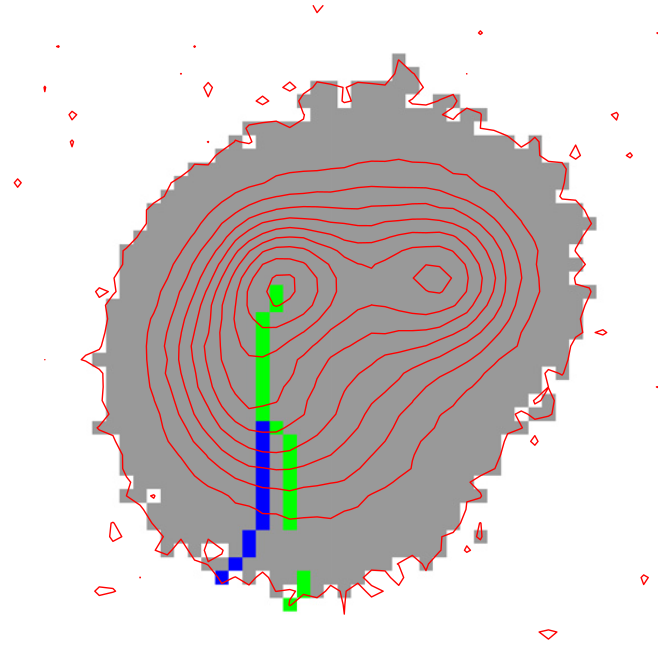
\includegraphics[width=6cm]{fw}
\caption{Dos rutas de ascenso de FellWalker en data 2D (Fuente: \cite{Berry})}
\label{fig:fw}
\end{figure}

En las comparaciones realizadas por Watson \cite{Watson} y el mismo Berry \cite{Berry}, ambos concluyen que FellWalker es un algoritmo más robusto en cuanto a los resultados que obtiene, en comparación a ClumpFind. En general ClumpFind tiende a ser muy sensible a sus parámetros de entrada y fragmenta los clumps más de los debido. 





\section{SexTractor}






\section{Dendrogramas}
Como se explicó en la introducción, uno de los aspectos más importantes para comprender el proceso de formación de estrellas en la nubes moleculares, es entender la relaciones jerárquicas existentes entre los distintos núcleos densos o clumps de la nube. Para ello Rosolowsky et al. \cite{Rosolowsky} propone organizar las clumps encontrados en una estructura de tipo árbol, denominada \textit{dendrograma}.

El enfoque es distinto a los algoritmos de segmentación local como ClumpFind y FellWalker, pues este propone realizar un seguimiento de las estructuras presentes sobre un rango de escalas. De modo similar a ClumpFind, este computa isosuperficies de los cubos de datos que representan a la nube, descomponiendo iterativamente tales isosuperficies en otras de menor tamaño, generando un catálogo de regiones que se almacenan en una estructura de árbol (Figura \ref{fig:dendro}). De esto modo, cada punto del dendrograma corresponde a un volúmen específico en dentro del cubo de datos, definido por la isosuperficie que lo acota.  

\begin{figure}[htpb!]
\centering
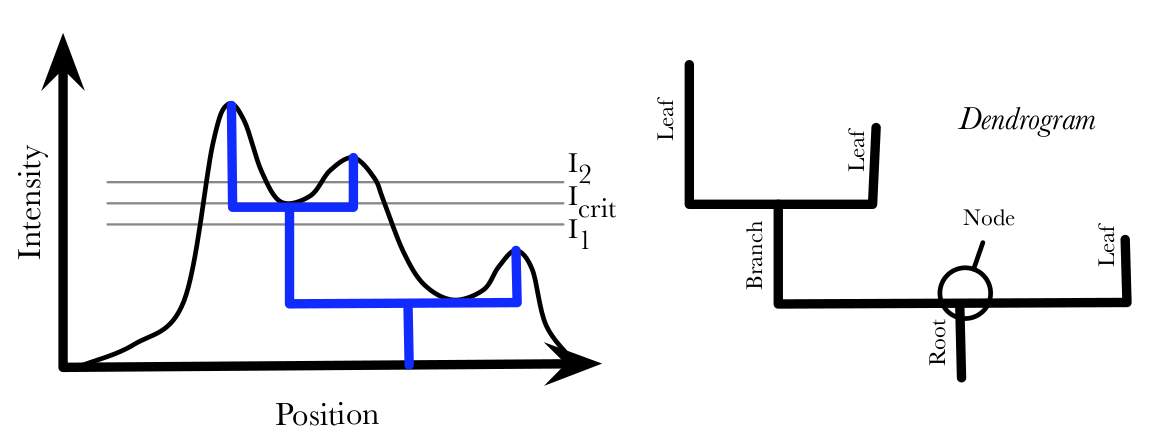
\includegraphics[width=12cm]{dendro}
\caption{Esquema de funcionamiento de Dendrogramas. \textit{Thresholding} al nivel $I_1$ produce un sólo objeto, mientras que al hacerlo a $I_2$ permite identificar dos. (Fuente: \cite{Rosolowsky})}
\label{fig:dendro}
\end{figure}





\section{Cálculo Variacional}
El cálculo variacional también conocido como cálculo de variaciones, es un campo muy antiguo (y por lo tanto muy estudiado) que trata acerca de la minimización de \textit{Funcionales}. Formalmente un funcional $\mathcal{U}$ es una correspondencia que asigna a cada función $f \in \mathcal{F}(\Omega \rightarrow \mathbb{C})$ un valor en un cuerpo escalar $\mathcal{K}$. Los funcionales son usualmente expresados como integrales definidas, involucrando a la función en cuestión y sus derivadas, como por ejemplo:
\begin{align}
    \mathcal{U}(f) = \int_{\Omega} L\left(\mathbf{x}, f(\mathbf{x}), \nabla f(\mathbf{x}), \Delta f(\mathbf{x})\right) d \mathbf{x},
\end{align}
donde la función $L$ es usualmente conocida en este ámbito, como el \textit{Lagrangiano}, así mismo al funcional $\mathcal{U}$ se le llama \textit{Funcional de Energía}.

El cálculo variacional sigue las mismas ideas del cálculo tradicional, esto es, define un equivalente a la derivada de las funciones pero sobre los funcionales, conocidas como \textit{variaciones}. Igualando la primera variación o \textit{variación ge Gateaux} a cero, y bajo ciertas otras restricciones, es posible encontrar la función $f_0$ que minimiza la energía del funcional, dando como resultado una ecuación diferencial llamada \textbf{Ecuación de Euler-Lagrange}.

De este modo se traslada el problema integral a un problema diferencial, para el cuál es posible ocupar toda la maquinaria de métodos numéricos (\textit{Finite differences}, \textit{Finite Element Methods}, \textit{Collocation Methods}, \textit{Spectral Methods}, etc) para intentar resolverla.

Para un tratamiento más acabado y formal de la formulación del problema variacional existen gran cantidad de libros que se pueden consultar.  Dos buenas referencias son Logan \cite{Logan} y Aubert \cite{Aubert}.   



\subsection{\textsc{Aplicaciones del Cálculo Variacional}}
En las últimas décadas el cálculo variacional ha venido sido utilizado como una potente herramienta para resolver múltiples problemas de minimización. Una de las áreas que más ha explotado esta herramienta es precisamente la del Procesamiento de Imágenes (\textit{Image Processing}). Tal como expone Aubert \cite{Aubert} dependiendo del problema a tratar, es posible construir un funcional acorde, de modo que su minimización permita alcanzar distintos objetivos en cuanto a procesamiento de imágenes. En lo que sigue se describen algunas de las aplicaciones principales en imágenes.

\begin{enumerate}
    \item \textsc{Denoising}. \\ \textbf{Objetivo:} Encontrar una aproximación \textit{suave} de la imagen, que por medio de este suavizamiento elimine el ruido en las zonas donde este se encuentre presente.
    \begin{figure}[htpb!]
    \centering
    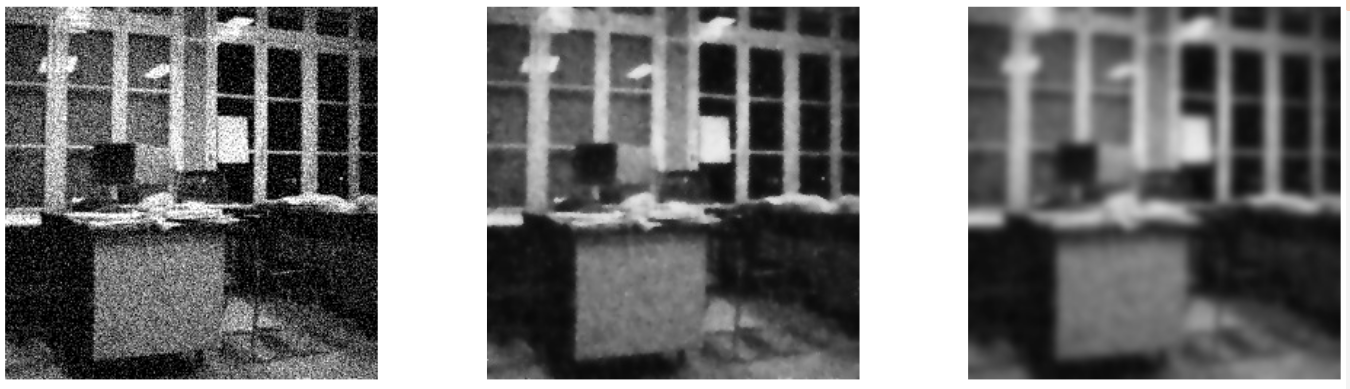
\includegraphics[width=11cm]{denoising}
    \caption{Proceso de \textit{denoising} por cálculo variacional}
    \label{fig:dendro}
    \end{figure}

    \item \textsc{Restoration}. \\ \textbf{Objetivo:} Encontrar una aproximación de una imagen con errores (zonas sin datos por ejemplo), que reconstruya estas zonas con errores de una manera \textit{suave}.
    \begin{figure}[htpb!]
    \centering
    
\includegraphics[width=8cm]{restoration}
    \caption{Proceso de \textit{restoration} por cálculo variacional}
    \label{fig:dendro}
    \end{figure}

    \item \textsc{Segmentation}. \\ \textbf{Objetivo:} Encontrar una curva cerrada \textit{suave}, entre un objeto de la imagen y el fondo.
     \begin{figure}[htpb!]
    \centering
    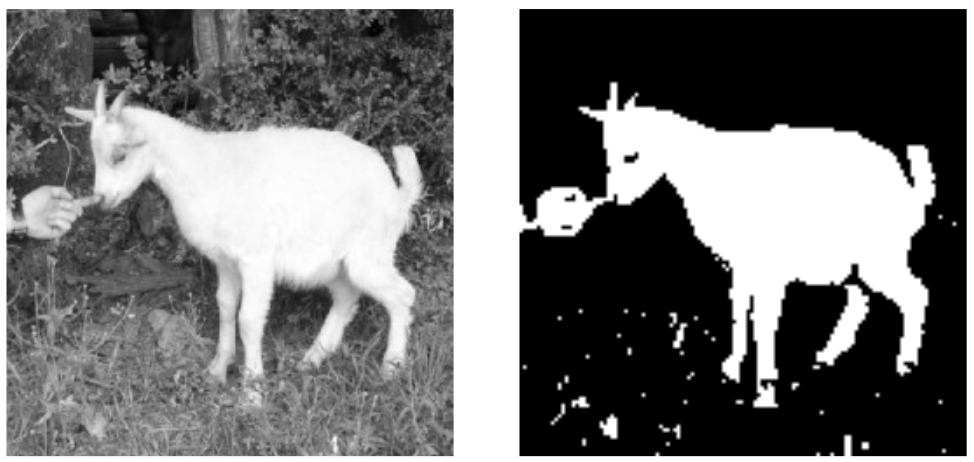
\includegraphics[width=8cm]{segmentation}
    \caption{Proceso de \textit{segmentation} por cálculo variacional}
    \label{fig:dendro}
    \end{figure}

    \item \textsc{Registration}. \\ \textbf{Objetivo:} Encontrar un campo de deformación, que permita hacer calzar una imagen de template y un imagen de entrada.
    \begin{figure}[htpb!]
    \centering
    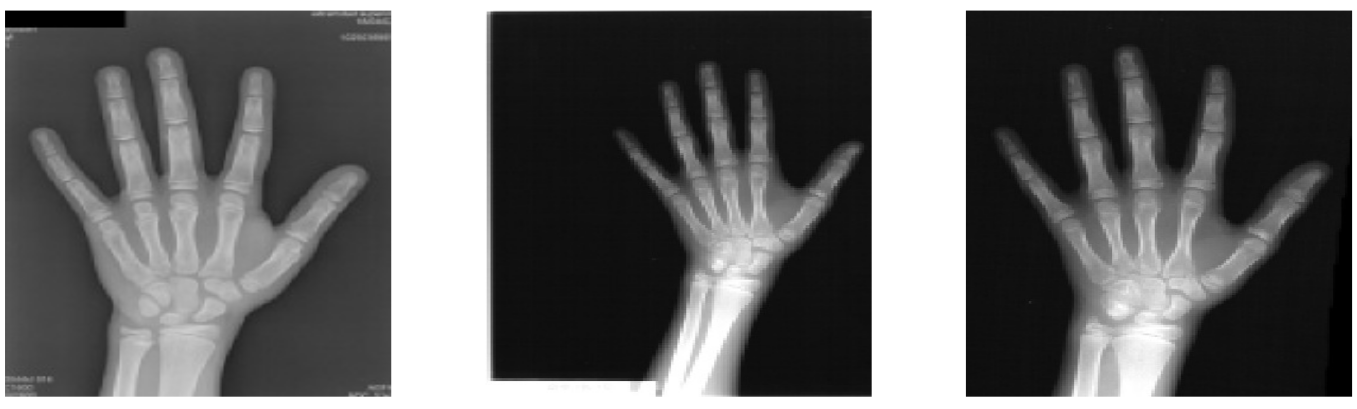
\includegraphics[width=11cm]{registration}
    \caption{Proceso de \textit{registration} por cálculo variacional}
    \label{fig:dendro}
    \end{figure}
\end{enumerate}

Para los dos primeros (\textit{denoising} y \textit{restoration}) el funcional de energía a minimizar tiene la forma general siguiente:
\begin{align}
    E(\mathbf{u}) = \int_{\Omega} \underbrace{D(\mathbf{u})}_{\text{Data term}} + \underbrace{S(\mathbf{u})}_{\text{Smoothing term}} + \underbrace{T(\mathbf{u})}_{\text{Domain specific term}} d\mathbf{x},
\end{align}
en donde cada término del \textit{Lagrangiano} cumple un objetivo específico: 1) $D$, que la solución sea cercana a la data de entrada, 2) $S$, que la solución sea suave, 3) $T$, que se cumplan restricciones propias del problema.

Las formulaciones del funcional a minimizar para los dos siguientes son más complicadas y requieren de un mayor análisis. Estas pueden ser consultadas en \cite{Aubert}.



\section{Gaussian Mixture Reduction}